\section{Attacco con ricerca lineare}

In un attacco di tipo password spraying esistono due entità, il database e il file con le password da testare, che vanno confrontati tra di loro. L'operazione di confronto è molto simile a un operazione di ricerca, infatti il database può essere visto come una lista utente-hash in cui si vuole controllare quali di questi hash sono contenuti nella lista delle password. Per cui ipoteticamente i passi che un algoritmo deve eseguire sono:
\begin{itemize}
    \item Caricare in memoria il file del database 
    \item Caricare in memoria il file delle password
    \item Calcolare l'hash della password correntemente in esame 
    \item Per ogni coppia nella lista del database controllare se esistono uno o più hash che corrispondono a quella password (al suo hash)
\end{itemize} 

In forma algoritmica questi passi si possono scrivere come
\begin{lstlisting}
    database = load_database()
    passwords = load_passwords()
    foreach word in passwords do {
        pwhash = hash(word)
        for i in 0..database.len {
            if pwhash == database[i].hash do{
                notify_password(word,database[i].user,database[i].password)
            }
        }
    }
\end{lstlisting}
Per analizzare questo semplice caso è opportuno introdurre le seguenti variabili
\begin{itemize}
    \item $H(X)$ numero di istruzioni necessarie per eseguire l'hashing della stringa x
    \item $C(X,Y)$ numero di istruzioni necessarie per eseguire una comparazione tra due stringhe 
    \item $L(X)$ numero di istruzioni necessarie per caricare una stringa dal disco 
\end{itemize}

si può stimare il tempo di calcolo come $T_{comp}=H(K)+C(N,K)$ \footnotemark[1] dove K è l'insieme delle password e N è l'insieme di coppie utente-hash nel file del database. Analogamente il tempo richiesto per effettuare le operazioni di comunicazione, in questo caso sono le operazioni di caricamento dei file, può essere stimato come $T_{comm}=L(K) + L(N)$. Se si mette tutto insieme $T(N,K)=H(K)+C(N,K)+L(K)+L(N)$ si può descrivere il problema in termini di complessita:
$T(N,K)=K+NK+K+N=NK + 2K + N$. 

\footnotetext[1]{Durante la trattazione si commetterà un piccolo abuso di notazione, le funzioni che accettano singole stringhe riportando il numero di istruzioni necessarie accetteranno anche insiemi di stringhe, per cui ad esempio $H(K)$ sarà il numero di istruzioni necessario ad effettuare l'hashing di tutto l'insieme delle password}


\subsection{Ricerca Lineare con architettura main worker}
L'architettura più semplice a cui si può pensare è sostanzialmente la classica main-worker, in cui più nodi , detti worker, che eseguono i task, in questo caso il confronto tra stringhe, vengono coordinati nelle loro operazioni da un main che distribuisce loro i dati su cui i task vengono effettuati. In pseudocodice si traduce facilmente in 

\begin{lstlisting}
    database = load_database()
    password = load_password()
    foreach pw in password do in parallel{
        pwhash = hash(pw)
        for i in 0..database.len do{
            if pwhash == database[i].hash{
                notify_password(pw,database[i].user,database[i].hash)
            }
        }
    }
\end{lstlisting}

Questo pseudocodice, molto generico, lancerebbe semplicemente la ricerca della password corrente in parallelo alle altre su tutte il database. Con lo scopo di analizzare in maniera più approfondita il problema con un approccio più distribuito si può riscrivere come\footnotemark[2]

\begin{lstlisting}
    rank = world().rank 
    if rank is root{
        database = load_database()
        password = load_password()
        broadcast(password, password.size)
        scatter(database, database/world.size)
    }
    else{
        password
        broadcast(password, password.size)
        database 
        scatter(database, database/world.size)
        foreach pw in password{
            pwhash = hash(pw)
            for i in 0..database.len do{
                if pwhash == database[i].hash{
                    notify_password(pw,database[i].user,database[i].len)
                }
            }
        }
    }
\end{lstlisting}

Che è un pò meno generale ma modella un pò meglio un ambiente di computazione distribuita oltre che parallela. In questo caso, l'algoritmo lavora in modo piuttosto semplice, prima di tutto si distribuisce una copia del file con le password a tutti i worker. Poi si divide in pezzi equamente grandi il file del database e lo si distribuisce tra i worker, a questo punto si effettua la comparazione e quando si incontra una password la si notifica. 

\begin{figure}[H]
    \centering
    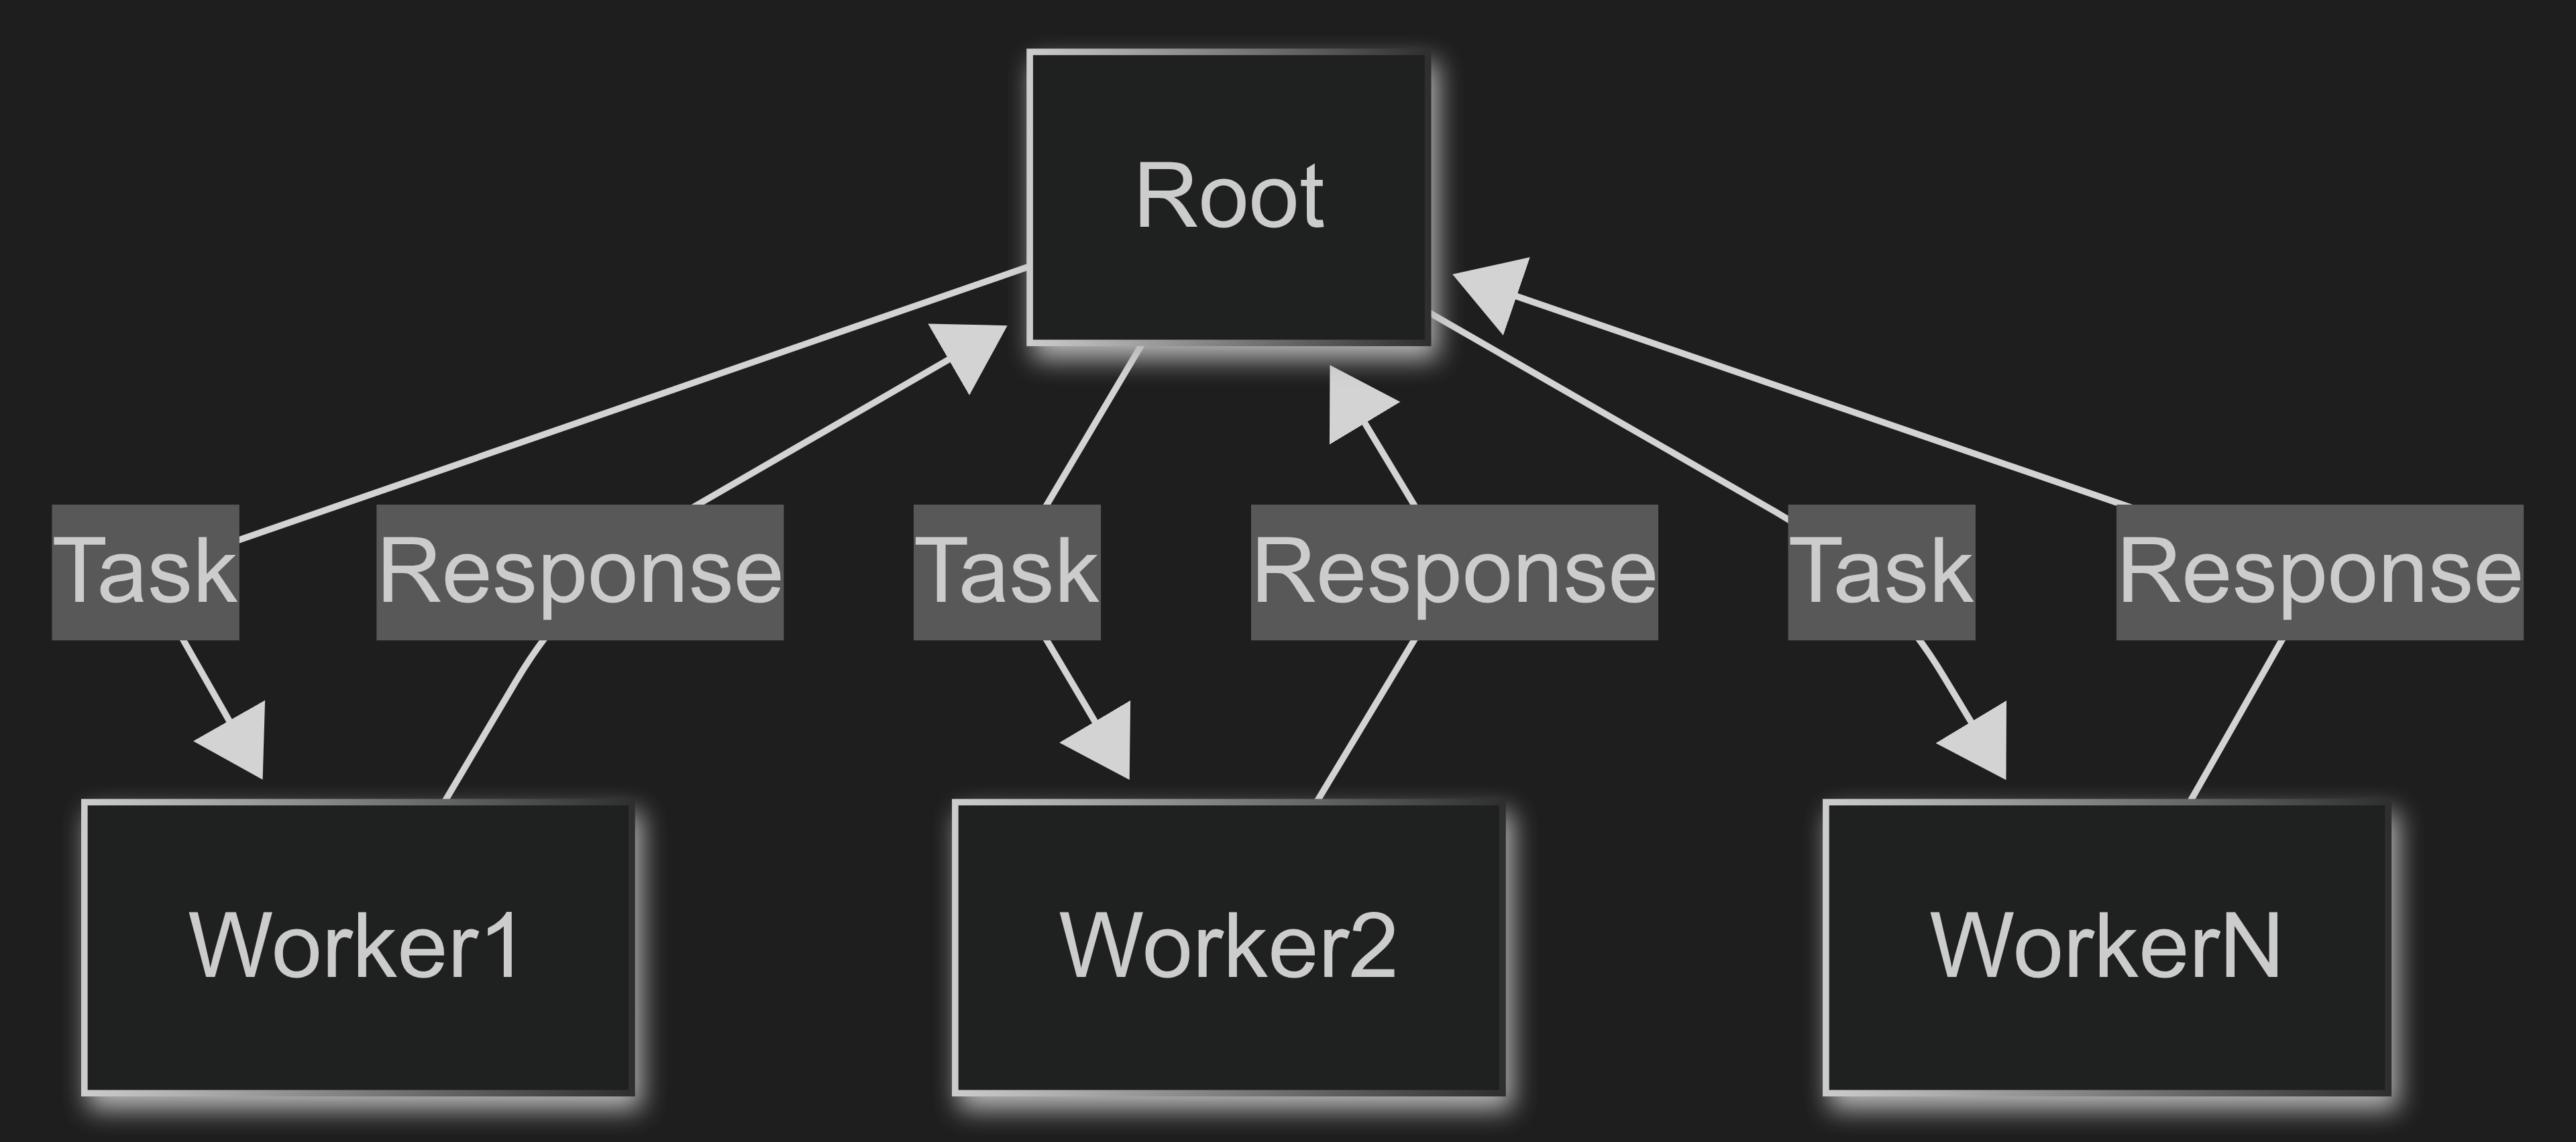
\includegraphics[width=0.6\textwidth]{images/main_worker_diagram.png}
    \caption{Architettura main worker proposta per il problema}
\end{figure}


\footnotetext[2]{World si riferisce alla variabile che permette di accedere al comunicatore globale di MPI}
\subsubsection{Speedup, Efficienza e CC Ratio}
Supponendo di assegnare le seguenti variabili 
\begin{itemize}
    \item P : il numero di esecutori 
    \item $S(X)$: il tempo necessario a trasmettere un elemento da un nodo all'altro, che è dipendente dalla dimensione dell'elemento 
\end{itemize}
Si può derivare il tempo di comunicazione $T_{comm}(P,N,K)=L(K)+L(N) +S(K)+S(\frac{N}{P})*P$ e il tempo di computazione effettivo 
$T_{comp}(P,N,K)=\frac{H(K)}{P}+C(\frac{N}{P},K)$ da cui si può ottenere il tempo totale di esecuzione
$$ 
T(P,N,K)=L(K)+L(N)+S(K)*P+S(\frac{N}{P})*P + \frac{H(K)}{P}+C(\frac{N}{P},K)
$$ 
Se si vuole analizzare questo modello con un approccio più standard, è possibile passare a BSP in modo piuttosto semplice assegnando opportunamente le seguenti varaibili 
\begin{itemize}
    \item $w = \frac{H(K)}{P} + C(\frac{N}{P},K)$ = numero di istruzioni che ogni processore dovrà eseguire, per questo problema è omogeneo
    \item $h=S(K)*P+S(\frac{N}{P})*P$ = latenza dovuta al numero di word da trasmettere 
    \item g ed l dipendono dall'hardware  
\end{itemize}
Il risultato è la seguente formula $T=w+gh+l$ che è la forma prevista dal modello BSP. 
\begin{itemize}
    \item Lunghezza media di una password : 16 caratteri 
    \item Istruzioni necessarie per inviare una word (g): 10 Flops
    \item Dimensione dell'hash : 32 byte 
    \item operazioni per SHA256 totali: 512 Flops
    \item Dimensione del dizionario delle password : $10^{6}$ stringhe 
\end{itemize}

La lunghezza media delle password è sicuramente più grande del normale, ma è stata scelta in modo da coprire anche quei database su cui è stata posta una policy molto stringente in termini di lunghezza delle password.Per ricavare g si è eseguito un semplice programma sul cluster di hpc4ai\cite{hpc4ai} che invii diverse word da 64 bit tra un nodo e l'altro, avendo poi ricavato il tempo medio si è calcolato il numero di flops necessari usando il modello del processore, Intel Xeon E5-2697V4, partendo dalla capacità di calcolo, approssimando per comodità il risultato per eccesso a 10. Il numero di operazioni necessarie invece per calcolare un blocco da 64 byte in SHA256 con 64 round è $SHA_{ops}=64*(6+2)$ dove 6 sono le operazioni logiche AND, OR, XOR, NOT, shift, rotate a cui il blocco viene sottoposto mentre 2 sono le due addizioni modulari $\mod 2^{32}$ che vengono compiute dall'algoritmo, per cui per ogni blocco sono necessarie 512 operazioni. L invece contiene tutta la parte dovuta all'inizializzazione della comunicazione e anche al caricamento dal disco dei file necessari.

\begin{figure}[H]
    \centering
    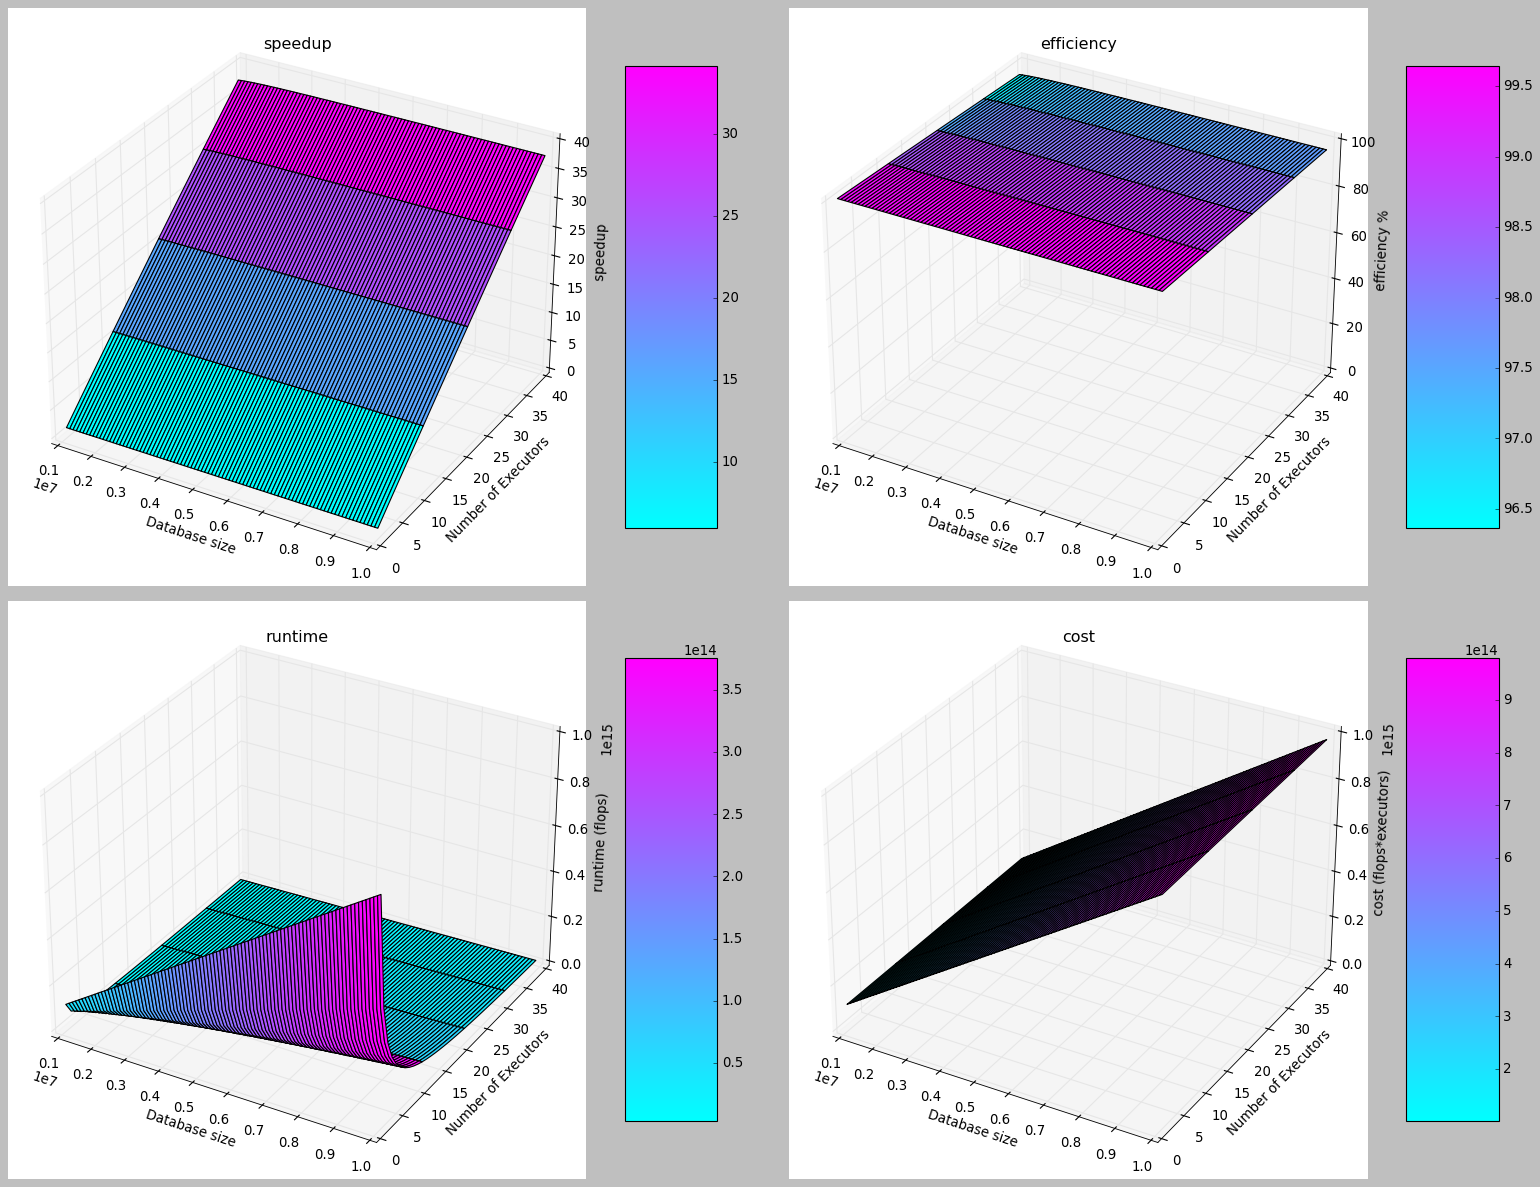
\includegraphics[width=0.9\textwidth]{images/mainworkerlinear.png}
    \caption{Misure ottenute dalla simulazione sul caso main worker}
\end{figure}

Il grafico mostra che l'algoritmo scala linearmente in base agli esecutori presenti nella rete, che è ciò che ci si aspetta da un algoritmo embarassingly parallel come questo, nonostante la sua semplicità questa soluzione offre diversi vantaggi:
\begin{itemize}
    \item è molto semplice da implementare 
    \item il numero di messaggi da scambiare durante l'esecuzione è molto basso
    \item i nodi non richiedono sincronizzazione una sincronizzazione esplicita 
\end{itemize}
purtroppo presenta uno svantaggio piuttosto importante, uno dei due insiemi va condiviso in copia tra i nodi, vista la notevole dimensione dei database è più facile condividere in copia il file delle password. Per cui se si vuole trattare il problema come un flusso costante di dati lo si potrà fare solo con il database. Il grafico mostra che si possono chiaramente aggiungere altri esecutori ed è un passo necessario per osservare fino a che punto ci si può spingere con questa soluzione 

\begin{figure}[H]
    \centering
    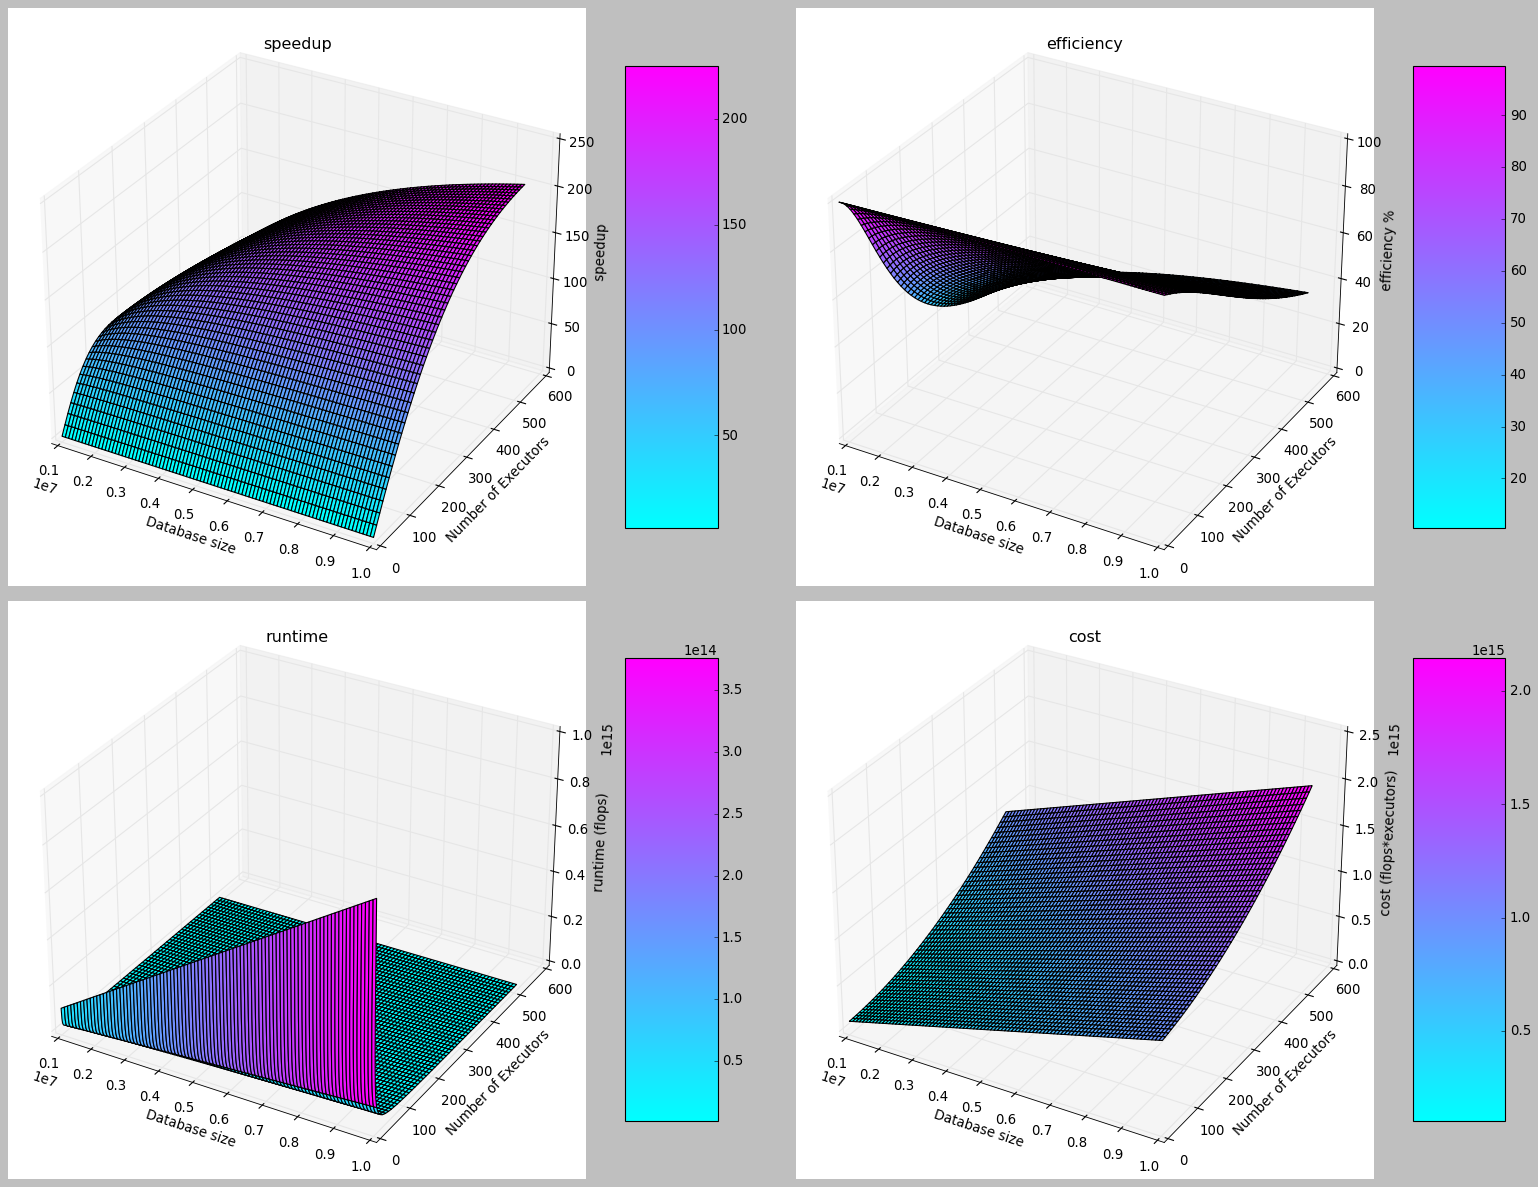
\includegraphics[width=0.9\textwidth]{images/mainworkermany.png}
    \caption{Misure ottenute dalla simulazione con più di 100 esecutori}
\end{figure}

Il grafico mostra subito che si ottiene una riduzione notevole del runtime entro i primi 100 esecutori, difatti si vede che l'efficienza decresce notevolmente superata quella soglia. 
\subsection{Ricerca con architettura ad anello}

Nel caso del main worker si è costretti a passare almeno uno dei due file in copie ai diversi nodi. A meno di non assicurarsi con metodi più o meno complicati, che ogni porzione del file di password sia stata comparata con ogni porzione del database in circolazione tra i nodi. In alternativa, si può adottare un'architettura con topologia ad anello ($N \to N+1 \pmod{P}$). In questo modello, il dizionario delle password viene suddiviso tra i nodi, mentre i blocchi del database "scorrono" attraverso la pipeline. Ad ogni stadio, un blocco di dati viene confrontato con il set di password locale, realizzando un confronto completo dopo un intero ciclo dell'anello.


\begin{figure}[H]
    \centering
    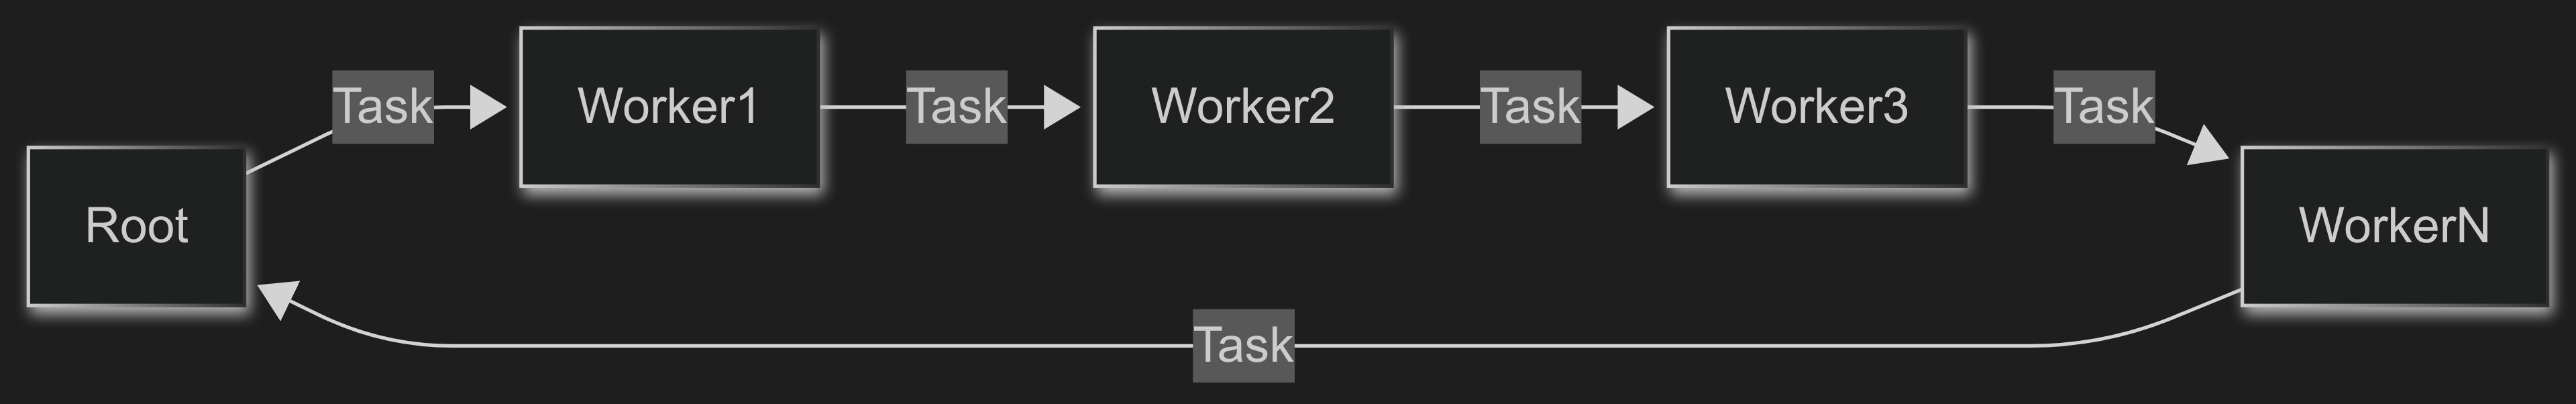
\includegraphics[width=0.6\textwidth]{images/pipeline_diagram.png}
    \caption{Architettura ad anello}
\end{figure}

In questa architettura, il primo passo è distribuire le password da testare ai vari nodi, dopodichè si comincia distribuendo il primo frammento del database al primo nodo, che comincierà il processamento e lo passerà al nodo successivo. Esistono due momenti transitori in questa architettura, il primo è all'inizio , quando il primo frammento di database viene dato al nodo di testa che lo dovrà passare allo stadio successivo e così via, fintanto che questo frammento non avrà percorso tutta la pipeline i nodi che non lo hanno ancora ricevuto non saranno ancora attivi, alla fine invece si verificherà il processo opposto, ossia man mano che l'ultimo frammento di database attraversa l'anello i vari nodi si disattiveranno, sostanzialmente buttando via tempo di esecuzione. Nonostante questo difetto, che è fortemente dipendente dalla lunghezza della pipeline, si ottiene un vantaggio sostanziale in termini di spazio occupato dal database e dalle password perchè non è più necessario che ogni nodo abbia in copia almeno uno dei due file, ma solo una porzione. In pseudocodice

\begin{lstlisting}
    rank = world().rank 
    if rank is root{
        password = load_password()
        database = load_database()
        datavector = split(database, world().size - 1)
        for i in 1..world.size() do{
            send(datavector[i],i)
        }
        tasks = split(password, world().size -1)
        for task in tasks do{
            send(task,rank+1,tasktoken)
        }
        send(rank+1,terminationtoken)
    }
    else{
        database = recv(root)
        while !terminationtoken{
            token = recv(rank-1)
            if token is tasktoken{
                for password in token.passwords do{
                    pwhash = hash(password)
                    for i in 0..database.len{
                        if pwhash == database[i].hash{
                            notify_password(password,database[i].user,database[i].hash)
                        }
                    }
                }
                send(rank+1,tasktoken)
            }
            if token is terminationtoken{
                break
            }
        }
    }
\end{lstlisting}

Per capire meglio se questo approccio possa essere più o meno vantaggioso rispetto al precedente è necessario modellare opportunamente il problema, avendo cura di trattare il periodo transitorio, che può essere visto come una somma di tempi, se si prende $T_{task}$ come tempo impiegato da un nodo a completare un task, allora il transitorio iniziale sarà $\sum_{i=1}^{P-1}(P-i)*T_{task}*2=\frac{(p-1)p}{2}T_{task}*2$. Il tempo che un nodo impiega a completare un task dipende dalla strategia adottata, se si decide di avere tanti task quanti sono i nodi, allora la sua dimensione sarà dipendente dalla grandezza dei due file e da quanti nodi sono presenti nell'anello. Viceversa , se invece si adottasse una politica per cui la grandezza del task è fissa, allora il numero di task presenti sarebbe dipendente esclusivamente dalla dimensione dei due file.

Ogni nodo per completare un task dovrà svolgere i seguenti passi:
\begin{enumerate}
    \item comparare gli elementi che ha a disposizione 
    \item ricevere e trasmettere il contenuto del task 
\end{enumerate}

Per cui questo tempo è rappresentabile, almeno nel primo caso in cui i task sono tanti quanti i nodi, come $T_{task} = T_{taskcomp} + T_{taskcomm}$ dove $T_{taskcomm} =S(\frac{N}{P})*2$ e $T_{taskcomp} = C(\frac{N}{P},\frac{K}{P})$. Ne consegue che si possono rappresentare il tempo di comunicazione e di computazione come:
$$ T_{comm} = L(K) + L(N) + S(K) + S(N) + T_{taskcomm}*P $$
$$ T_{comp} = \frac{T_{task}*P}{P} + \frac{(P-1)*P}{2}*T_{task} $$

Si considera quindi il tempo transitorio come tempo di computazione aggiuntivo. Con queste variabili si può scrivere:

$$
T(P)=T_{comm} + T_{comp}=  L(K) + L(N) + S(K) + S(N) + T_{taskcomm}*P + \frac{T_{taskcomp}*P}{P} + \frac{(P-1)*P}{2}*T_{task}
$$



\begin{figure}[H]
    \centering
    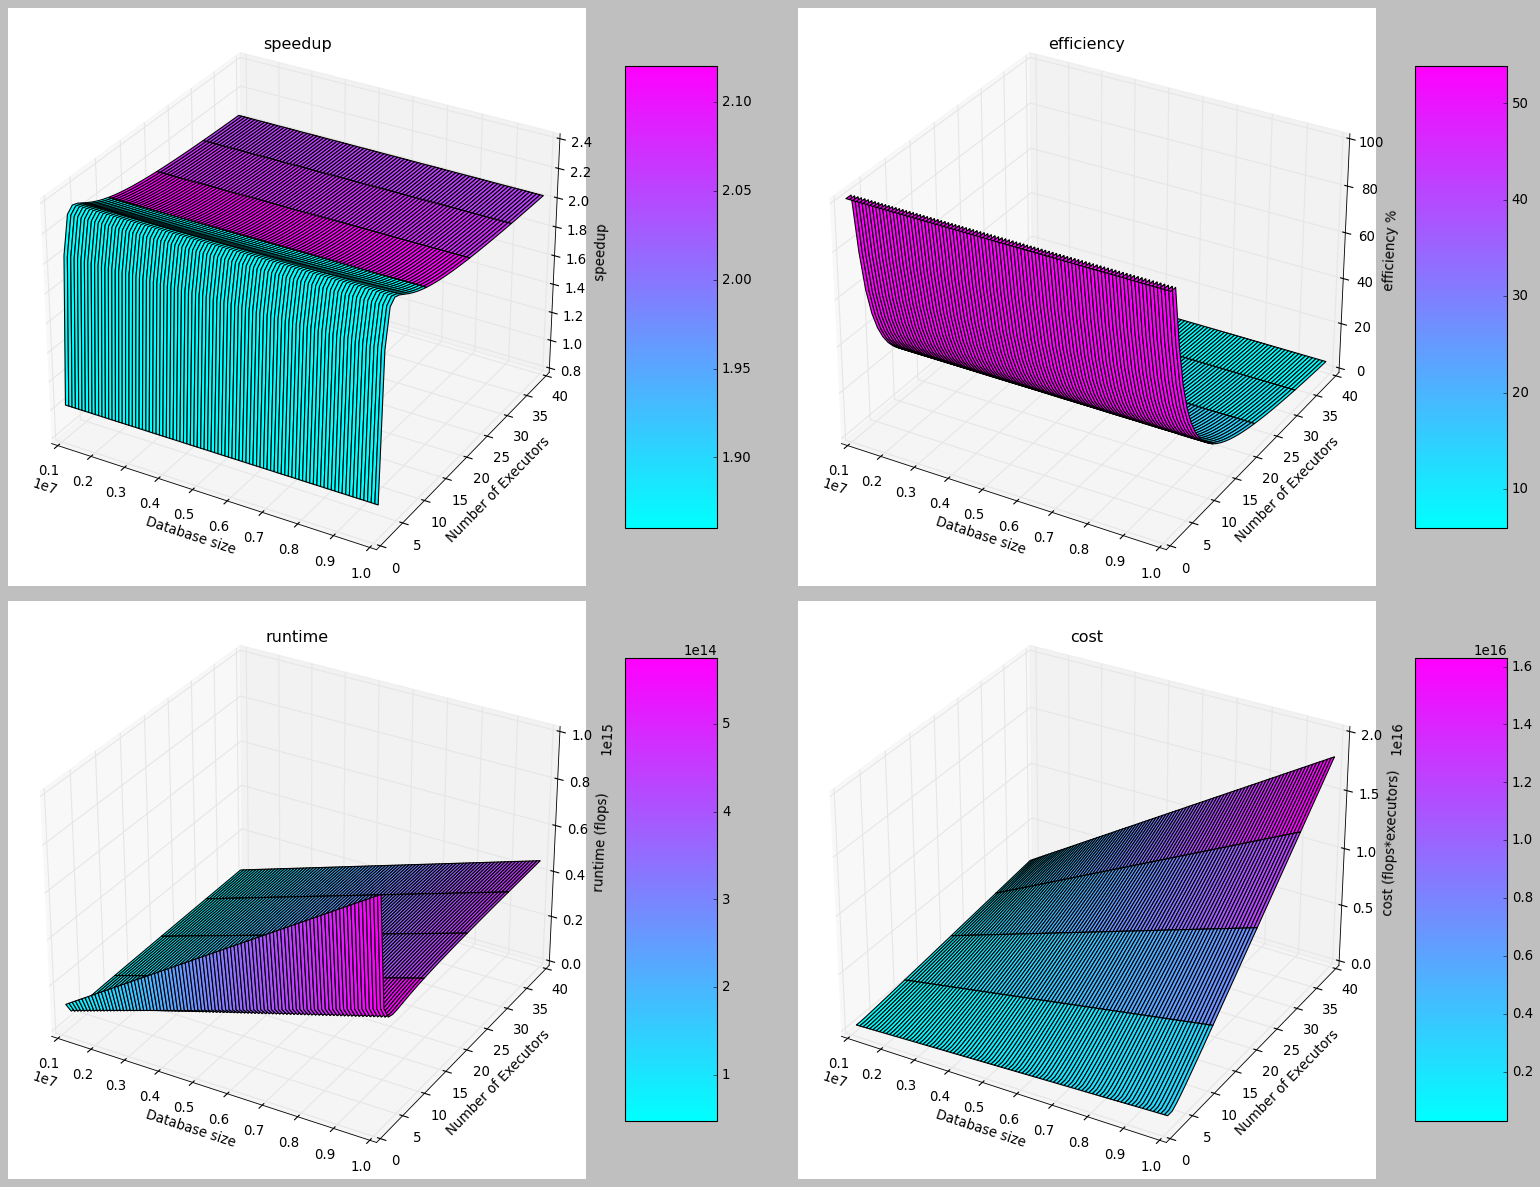
\includegraphics[width=0.8\textwidth]{images/pipelinelinear.png}
    \caption{speedup,costo,efficienza e cc ratio dell'architettura ad anello con numero di task fissi}
\end{figure}

La simulazione mostra che quest'architettura soffre parecchio il periodo transitorio iniziale, come ci si aspetta, poichè con questo approccio a task equamente distribuiti non si usino praticamente mai tutti gli esecutori, con la conseguenza che l'anello si riempirà del tutto per un breve momento prima di doversi svuotare nuovamente. 

Come accennato precedentemente una possibile miglioria può essere quella di introdurre dei task a dimensione fissa, opportunamente scelta per evitare di saturare troppo  l'I/O e ridurre i periodi transitori. Si supponga di assegnare a $T_s$ la dimensione massima del task, allora il numero di task da completare sarà $T_n(p)= \lceil \frac{T_s}{p} \rceil$, da cui si può ottenere una nuova definizione del tempo per completare un task $T_{task}=S(T_s)*2 + C(\frac{N}{P},T_s)$. A questo punto si può modificare leggermente l'espressione precedentemente usata per descrivere il tempo in 
$$T(P)=L(K) + L(N) + S(K) + S(N) + T_{taskcomm}*T_n(p) + \frac{T_{taskcomp}*T_n(p)}{P} + \frac{(P-1)*P}{2}*T_{task}$$ 


\begin{figure}[H]
    \centering
    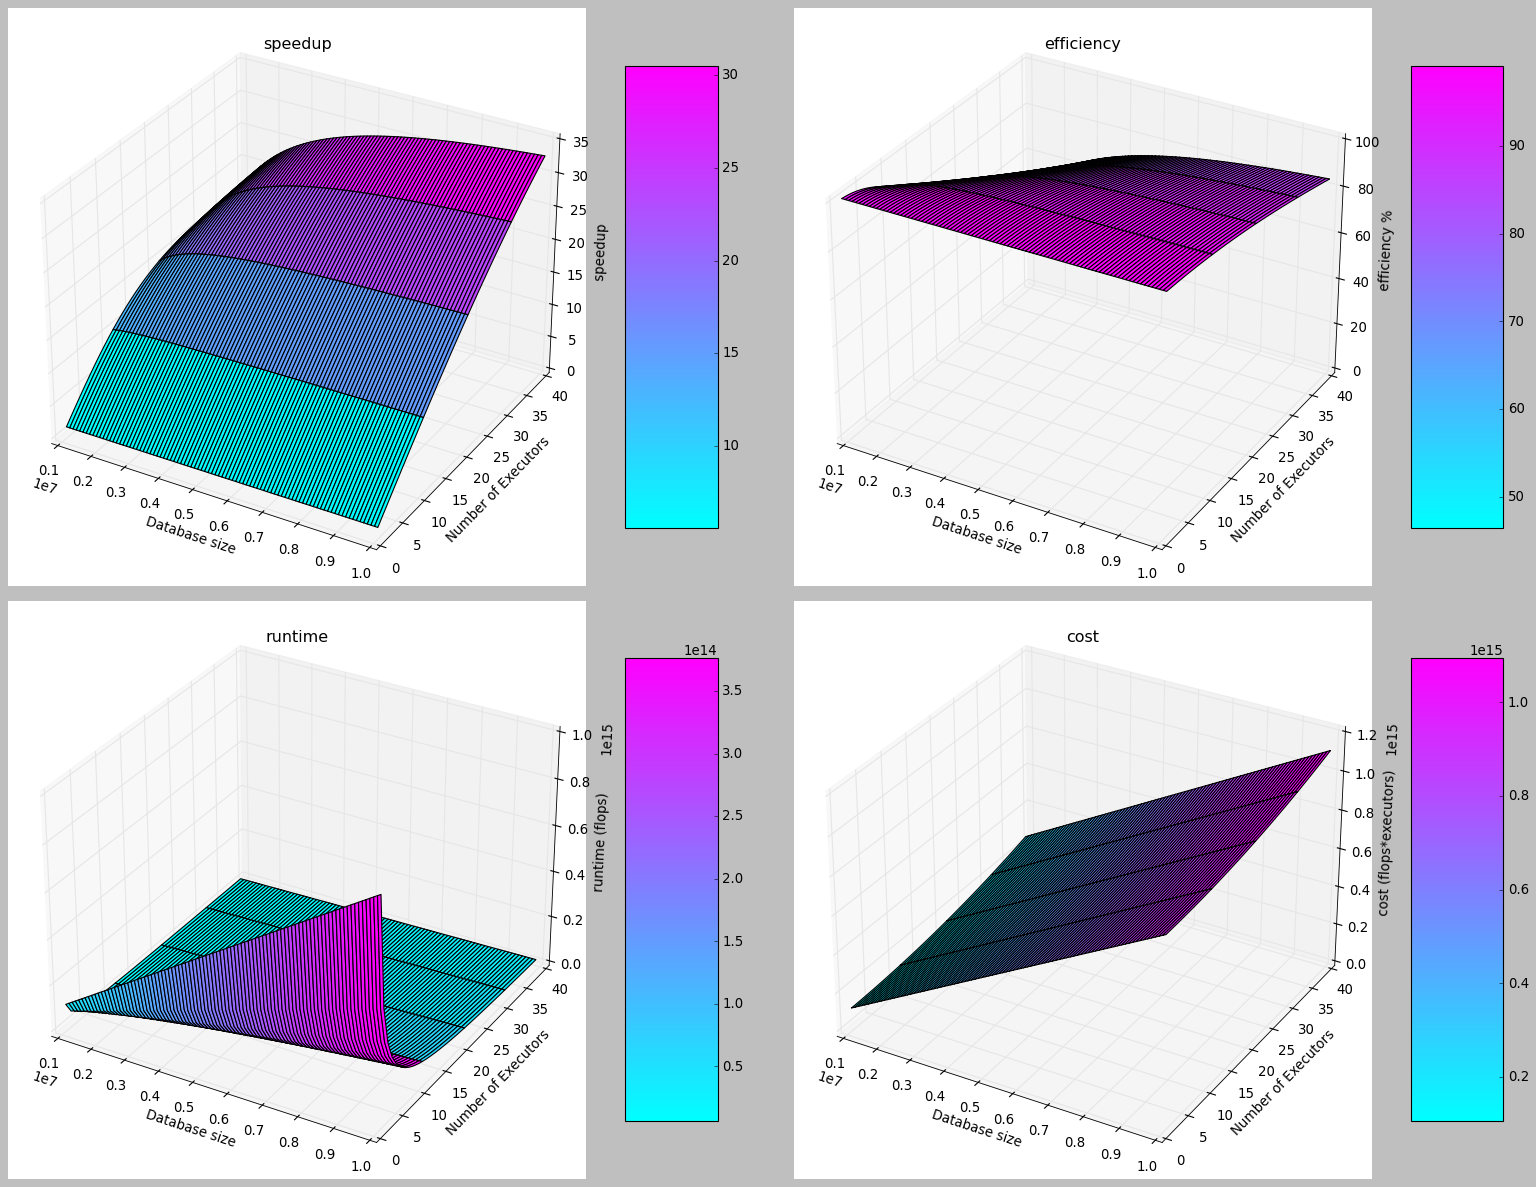
\includegraphics[width=0.8\textwidth]{images/pipelineblocked.png}
    \caption{speedup,costo,efficienza e runtime dell'architettura ad anello con task fissi grandi 2000 stringhe a blocco}
\end{figure}

Confronto al caso precedente, in cui erano presenti task di dimensione variabile a seconda degli esecutori questo caso presenta invece una buona performance. L'introduzione di una variabile aggiuntiva come la dimensione del task richiederebbe ovviamente più esecuzioni per poter effettuare uno scrutinio più approfondito, tuttavia empiricamente si è ottenuto che almeno a livello teorico la configurazione della grandezza del task impatta in modo completamente diverso l'esecuzione in base a quanti nodi sono disponibili, pertanto bisognerebbe effettuare diverse prove per capire se esistono eventualmente degli ottimi.


Questa architettura per quanto possa sembrare un poco più complicata da gestire, presenta il notevole vantaggio di poter suddividere tra gli esecutori tutti e due i file, ma non solo, nel caso in cui vi fosse uno dei due file notevolmente più grande dell'altro si può trattare questo ultimo come uno stream. Per esempio nel caso del database, che di solito è un file o in questo caso un flusso di dati molto più grande delle password, può essere fatto "scorrere" nella pipeline senza per forza conoscere le sue dimensioni effettive. Per altro questo metodo rispetto al precedente main worker, ha anche il vantaggio di consumare meno RAM, poichè non è necessario copiare uno dei due file da distribuire agli esecutori. 